% id: 85-e2
% book: 100발100중 3-2 중간 · 01 3-2 중간(삼각비·삼각비의 활용·원과 직선·원주각·부록)
% section: 서술형 문제
% figure: crop:fig-85-e2-2.png
% answer: (1) $30^\circ$ (2) $60^\circ$
% answer_source: 예제 모범답안
% variant_level: 0 (원본 전사)
% 이 파일은 build.mjs 가 items.json 에서 만든다. 고칠 때는 items.json 을 고친다.
\smash{\raisebox{1.5mm}{\dmkichul{100발100중 3-2 중간 85쪽 예제 2 · 예제}}}
\noindent\begin{minipage}[t]{0.58\linewidth}\vspace{0pt}\raggedright 그림에서 $\seg{BE}$는 원~$\pt{O}$의 지름이고 $\arc{BC}$의 길이는 $\arc{AB}$의 길이의 $4$배이다. $\angle\pt{ADB}=15^\circ$일 때, 다음 물음에 답하고, 그 과정을 서술하시오. \mbox{[5점]}\end{minipage}\hfill\begin{minipage}[t]{0.4\linewidth}\vspace{0pt}\centering 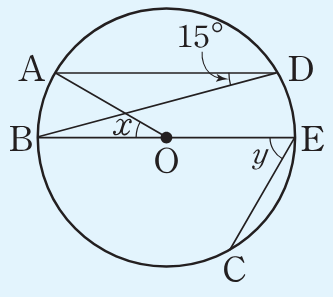
\includegraphics[width=79.8pt]{figures/fig-85-e2-2.png}\end{minipage}\par
\dmsubprob{1} $\angle x$의 크기를 구하시오. (2점)
\dmsubprob{2} $\angle y$의 크기를 구하시오. (3점)
